\section{Toiminta}
\subsection{Kokoukset}

\begin{figure}[htb]
	\begin{center}
		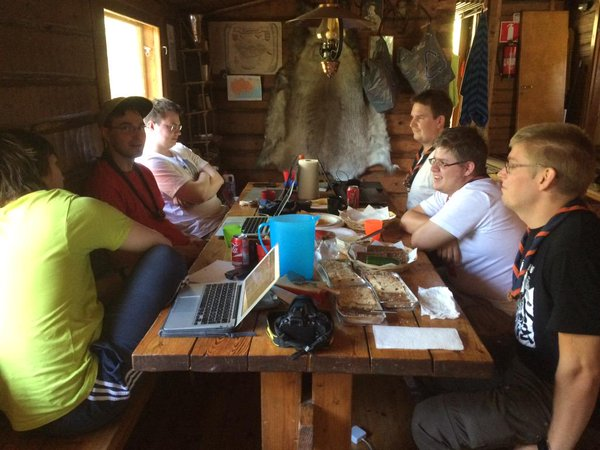
\includegraphics[height=7cm]{kuvat/kokous.jpg}
	\end{center}
	\captionsetup{labelformat=empty}
	\caption{\textbf{Toiminnansuunnittelua lippukunnan kämpällä.}}
\end{figure}


Ryhmät koontuivat omiin tapaamisiinsa viikoittain ja johtajat pitivät omia kokouksiaan tarpeen mukaan, esimerkiksi retkien suunnittelua varten. Kokouksista ja niiden määrästä lista alla:\\
\begin{center}
	\begin{tabular}{ l l }
		Vuosikokous & 1 kpl\\
		Vaalikokous & 1 kpl\\
		Hallituksen kokous & 9 kpl\\
		Poikasamoajat & 20 kpl\\
		Poikatarpojat & 20 kpl\\
		Poikasudenpennut & 50 kpl\\
		Tyttötarpojat & 25 kpl\\
		Tyttöseikkailijat & 25 kpl\\
		Tyttösudenpennut & 25 kpl\\
					 & \\
		\textbf{Yhteensä} & \textbf{176 kpl}\\
	\end{tabular}
\end{center}
Lisäksi vuoden mittaan on pidettu lukuisia muita pienempiä ja epävirallisia kokouksia, joissa on esimerkiksi suunniteltu toimintaa, retkiä tai kämppien kunnostusta.
\subsection{Leirit ja retket}
\subsubsection{Jouluretki}
Joulukuussa 2015 Helsingin Kotkat järjesti kaksi yötä kestäneen talviretki Tontun. Retkenjohtajina toimivat yhdessä Jukka Holopainen ja hänen kaksoisveljensä Pekka Holopainen. Retken teemana toimi tonttuilu ja viikonlopun aikana suunnistettiin, harjoiteltiin partio- ja kädentaitoja sekä kehitettiin lasten esiintymistaitoja. Lisäksi retkellä annettiin partiolupauksia jokaiselle ikäkaudelle. Retki oli johtajiensa PJ-lopputyö ja sille osallistui 11 johtajaa ja 26 retkeläistä.
\subsubsection{Kevätretki}
Huhtikuussa 2016 järjestettiin lippukunnan perinteinen keväretki, jonka johtajana toimi Adel Gatoui. Retkelle otettiin mukaan kaikki seikkailijat ja heitä vanhemmat HeKolaiset. Tämä johtui siitä, että retkellä ei ollut lainkaan sisämajoitusta ja siellä järjestetty pienoisvaellus oli suhteellisen pitkä. Mukana oli 9 johtajaa ja 16 retkeläistä.
\subsubsection{SuSe-leiri}
Tähän juduja kun leiri on pidetty.
\subsubsection{Roihu 2016}
Tähän setti Roihun jälkeen.
\subsubsection{Ryhmien retket}
Lippukunnan ryhmät ja osastot retkeilivät seuraavasti:
\begin{center}
	\begin{tabular}{l l l}
		16.-18.10. & Poikasamoajat Willassa & 4 osallistujaa\\
		30.10.-1.11. & Tyttöseikkailijoiden retki & 10 osallistujaa\\
		11.-13.3. & Tyttöosaston retki & 21 osallistujaa\\
	\end{tabular}
\end{center}
\subsection{Muu toiminta}
\subsubsection{Kisat}
Helsingin Kotkaista oli edustajat lähes jokaisissa pääkaupunkiseudulla järjestetyissä partiotaitokilpailussa. Mainetta ja kunniaa ei niistä kummemmin niitetty, mutta niissä edustaneiden lippukuntalaisten partiotaidot kasvoivat ja kehittyivät henkisen kasvun ja partioaatteen ymmärtämisen ohella.
\subsubsection{Kurssit ja koulutus}
Lippukuntalaiset kävivät tällä toimikaudella poikkeuksellisen paljon johtajakoulutusta. Partionjohtajakurssilla ja ryhmänohjaajakurssilla oli molemmilla kaksi edustajaa. Ryhmänohjaajakurssi järjestettiin yhteistyössä Vuosaaren Vesipääskyjen ja Sipoonkorven Haltiat. Kurssi koostui kahdesta kaupunkitapaamisesta sekä maasto- ja kämppäviikonlopuista, joista viikonloppujen aikana suoritettiin myös partionjohtajakurssin johtamisharjoitteita. Osallistujia ryhmänohjaajakurssilla oli 15.
\subsubsection{Johtajahuolto}
Lippukunnan perinteisiin kuuluu myös johtajahuollon järjestäminen. Johtajisto käy aina perinteisesti Joulun alla keilaamassa, jonka jälkeen siirrytään illalliselle läheiseen ravintolaan. Johtajahuoltoa toteutettiin myös toiminnansuunnitteluviikonloppuna Nuuksiossa elokuun lopulla.
\subsubsection{Lupauksenannot}
Tärkeä osa partiotoimintaa on sen arvojen ja aatteiden tunnustaminen ja ymmärtäminen. Tätä varten on olemassa partiolupaus, joka annetaan lupauksenantotilaisuudessa lippukunnanjohtajalle. Tällä toimikaudella niitä järjestettiin kaksi kappaletta, yksi jouluretki Tontulla ja toinen maaliskuussa lippukunnan kololla.
\newpage

